%%%%%%%%%%%%%%%%%%%%%%%%%%%%% Define Article %%%%%%%%%%%%%%%%%%%%%%%%%%%%%%%%%%
\documentclass{article}
%%%%%%%%%%%%%%%%%%%%%%%%%%%%%%%%%%%%%%%%%%%%%%%%%%%%%%%%%%%%%%%%%%%%%%%%%%%%%%%

%%%%%%%%%%%%%%%%%%%%%%%%%%%%% Using Packages %%%%%%%%%%%%%%%%%%%%%%%%%%%%%%%%%%
\usepackage{ctex}
\usepackage{geometry}
\usepackage{graphicx}
\usepackage{pgfplots}
\usepackage{float}
\usepackage{minted}
\usepackage{hyperref}
\hypersetup{
  colorlinks=true,
  pdfstartview=Fit,
  pdfcreator={Shit},
pdfproducer={Big shit}}
%\usepackage{amssymb}
%\usepackage{amsmath}
%\usepackage{amsthm}
%\usepackage{empheq}
%\usepackage{mdframed}
%\usepackage{booktabs}
%\usepackage{lipsum}
%\usepackage{color}
%\usepackage{psfrag}
%\usepackage{bm}
%%%%%%%%%%%%%%%%%%%%%%%%%%%%%%%%%%%%%%%%%%%%%%%%%%%%%%%%%%%%%%%%%%%%%%%%%%%%%%%

% Other Settings

%%%%%%%%%%%%%%%%%%%%%%%%%% Page Setting %%%%%%%%%%%%%%%%%%%%%%%%%%%%%%%%%%%%%%%
\geometry{a4paper}

%%%%%%%%%%%%%%%%%%%%%%%%%%%%%%% Plotting Settings %%%%%%%%%%%%%%%%%%%%%%%%%%%%%
\usepgfplotslibrary{colorbrewer}
\pgfplotsset{width=8cm,compat=1.18}
%%%%%%%%%%%%%%%%%%%%%%%%%%%%%%%%%%%%%%%%%%%%%%%%%%%%%%%%%%%%%%%%%%%%%%%%%%%%%%%

%%%%%%%%%%%%%%%%%%%%%%%%%%%%%%% Title & Author %%%%%%%%%%%%%%%%%%%%%%%%%%%%%%%%
\title{实验五: SPARK SQL 基础编程方法二}
\author{胡嘉鑫 \and 102102145}
\date{\today}
%%%%%%%%%%%%%%%%%%%%%%%%%%%%%%%%%%%%%%%%%%%%%%%%%%%%%%%%%%%%%%%%%%%%%%%%%%%%%%%

\begin{document}
\maketitle
\tableofcontents

\section{实验目的}
\begin{itemize}
  \item 理解 SPARK 工作流程;
  \item 掌握 SPARK SQL 基础编程方法;
\end{itemize}

\section{实验平台}
\begin{itemize}
  \item OS: Linux
  \item Hadoop v3.1.3
  \item JDK v1.8
  \item Spark v3.4.0
\end{itemize}

\section{实验步骤}
\subsection{用户搜索前三名统计}
\subsubsection{Problem Description}
用户搜索日志记录文件为 UserLogHot.txt, 格式为日期, 用户 id, 商品, 用户区域,
搜索终端;
\begin{enumerate}
  \item 查询每天每用户点击某商品的次数, 输出到屏幕.
  \item 将用户每天点击商品的次数汇总累加,
    统计每用户在每天点击搜索每个商品的总次数,
    输出 JSON 格式文件, JSON 元数据格式如下:
    Date(日期)、UserID(用户 id)、Item(商品)、Count(该用户在当天点击该商品的次数)
  \item 统计出用户搜索每商品的前 $ 3 $ 名:
    用步骤 $ 2 $ 的 JSON 字符串, 构造DataFrame。
    在 Spark SQL 注册临时表, 使用窗口函数 row\_number 统计出每用户搜索每商品的前
    $ 3 $ 名, 将结果以 JSON 格式输出到屏幕或者文件。
\end{enumerate}

\subsubsection{Code}
\begin{center}
\begin{minted}[xleftmargin=5mm]{scala}
package net.homework

import org.apache.spark.SparkContext._
import org.apache.spark.sql.SparkSession
import org.apache.spark.sql.functions.{expr, col, row_number}
import org.apache.spark.sql.expressions.Window
import org.apache.spark.sql.types.{
  StructField, StructType,
  StringType, LongType, DoubleType
}
import org.apache.spark.sql.Row

import java.nio.file.Paths

object App {
  def main(args : Array[String]) : Unit = {
    val spark = SparkSession
      .builder()
      .appName("pro1")
      .getOrCreate()

      val cwd = Paths.get("").toAbsolutePath.toString
      val inputPath = s"file://${cwd}/input"
      val outputPath = s"file://${cwd}/output"

      val schema = new StructType(Array(
        new StructField("DATE", StringType, true),
        new StructField("USERID", StringType, true),
        new StructField("ITEM", StringType, true),
        new StructField("CITY", StringType, true),
        new StructField("PLATFORM", StringType, true)
      ))

      val df = spark.read
        .option("header", "false")
        .option("sep", "\t")
        .schema(schema)
        .format("csv")
        .load(s"${inputPath}/UserlogsHot.log")
      df.cache()

      // 查询每天每用户点击某商品的次数, 输出到屏幕.
      val query1 = df.groupBy("USERID", "DATE", "ITEM")
        .agg(expr("COUNT(*) AS CNT"))

      query1.cache()

      query1.collect()
        .foreach(println)

      // 将用户每天点击商品的次数汇总累加,
      // 统计每用户在每天点击搜索每个商品的总次数,
      // 输出 JSON 格式文件, JSON 元数据格式如下:
      // Date(日期)、UserID(用户 id)、Item(商品)、Count(该用户在当天点击该商品的次数)
      query1.write
        .format("json")
        .mode("overwrite")
        .save(s"${outputPath}/query1.json")

      // 统计出用户搜索每商品的前 $ 3 $ 名:
      // 用步骤 $ 2 $ 的 JSON 字符串, 构造DataFrame。
      // 在 Spark SQL 注册临时表, 使用窗口函数 row\_number 统计出每用户搜索每商品的前
      // $ 3 $ 名, 将结果以 JSON 格式输出到屏幕或者文件。
      val df1 = spark.read
        .option("inferSchema", "true")
        .format("json")
        .load(s"${outputPath}/query1.json")

      val windowSpec = Window.partitionBy("USERID")
        .orderBy(col("CNT").desc)
        .rowsBetween(Window.unboundedPreceding, Window.currentRow)

      val df2 = df1.withColumn("rn", row_number().over(windowSpec))
      df2.createOrReplaceTempView("df2_view")
      spark.sql("""
        SELECT * FROM df2_view
        WHERE rn BETWEEN 1 AND 3
      """)
        .write
        .format("json")
        .mode("overwrite")
        .save(s"${outputPath}/result.json")

      spark.stop()
  }
}
\end{minted}
\end{center}

\subsubsection{Result}
\begin{figure}[H]
  \begin{center}
    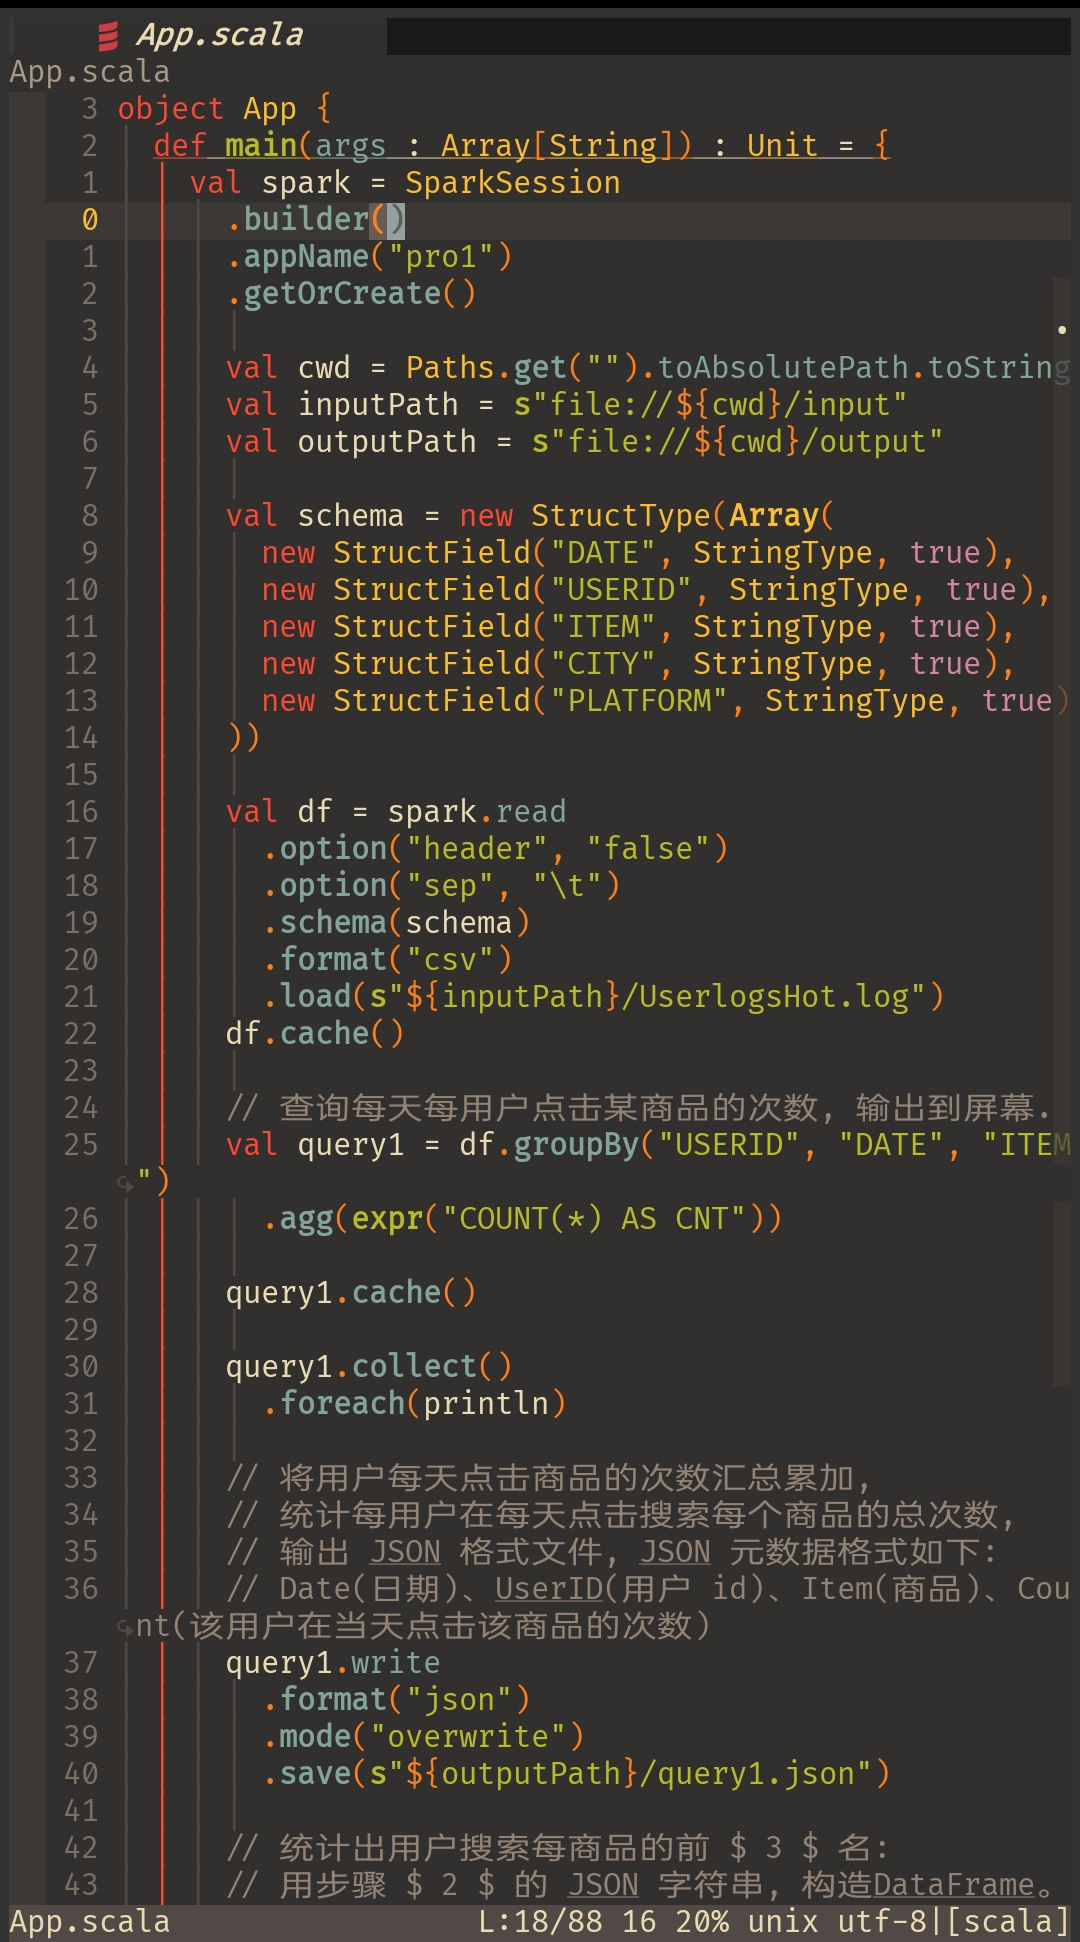
\includegraphics[width=0.65\textwidth]{./figures/1.jpg}
  \end{center}
  \caption{Code}
\end{figure}

\begin{figure}[H]
  \begin{center}
    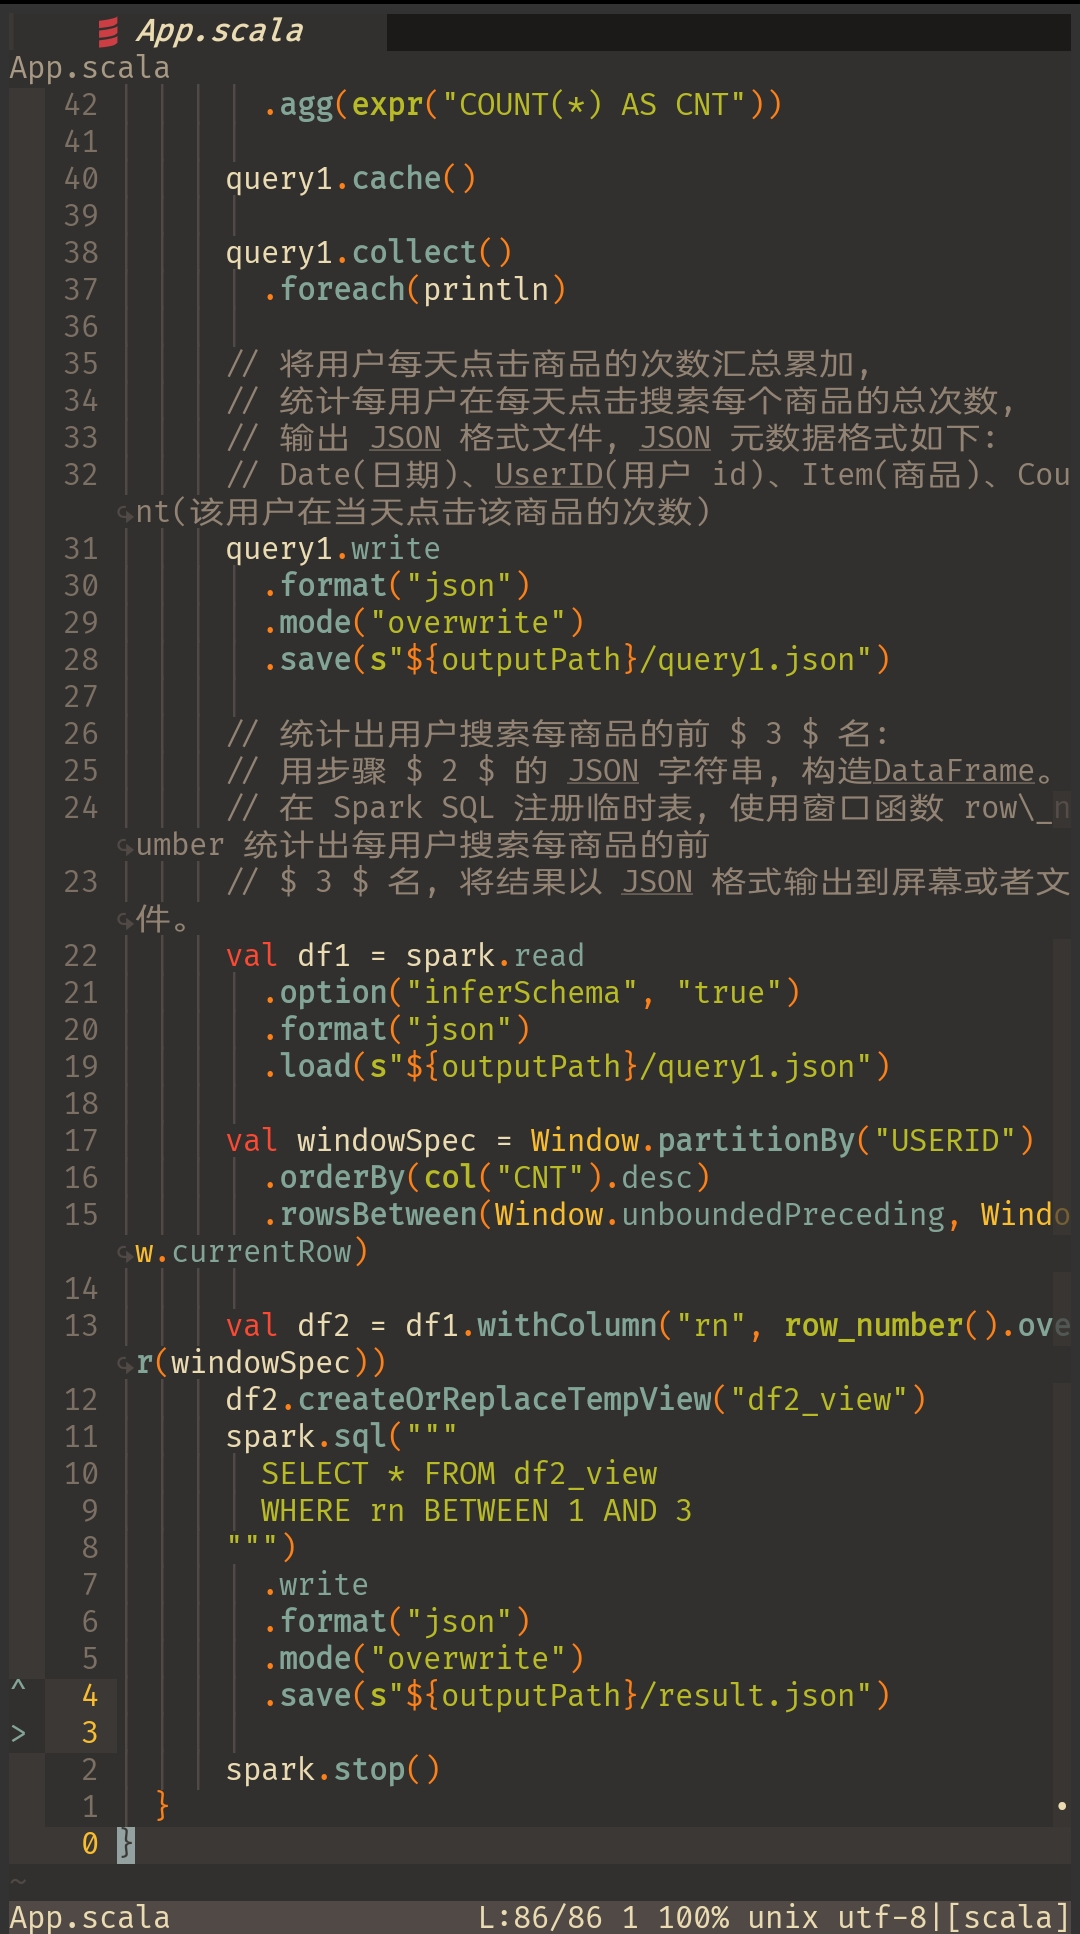
\includegraphics[width=0.65\textwidth]{./figures/2.jpg}
  \end{center}
  \caption{Code}
\end{figure}

\begin{figure}[H]
  \begin{center}
    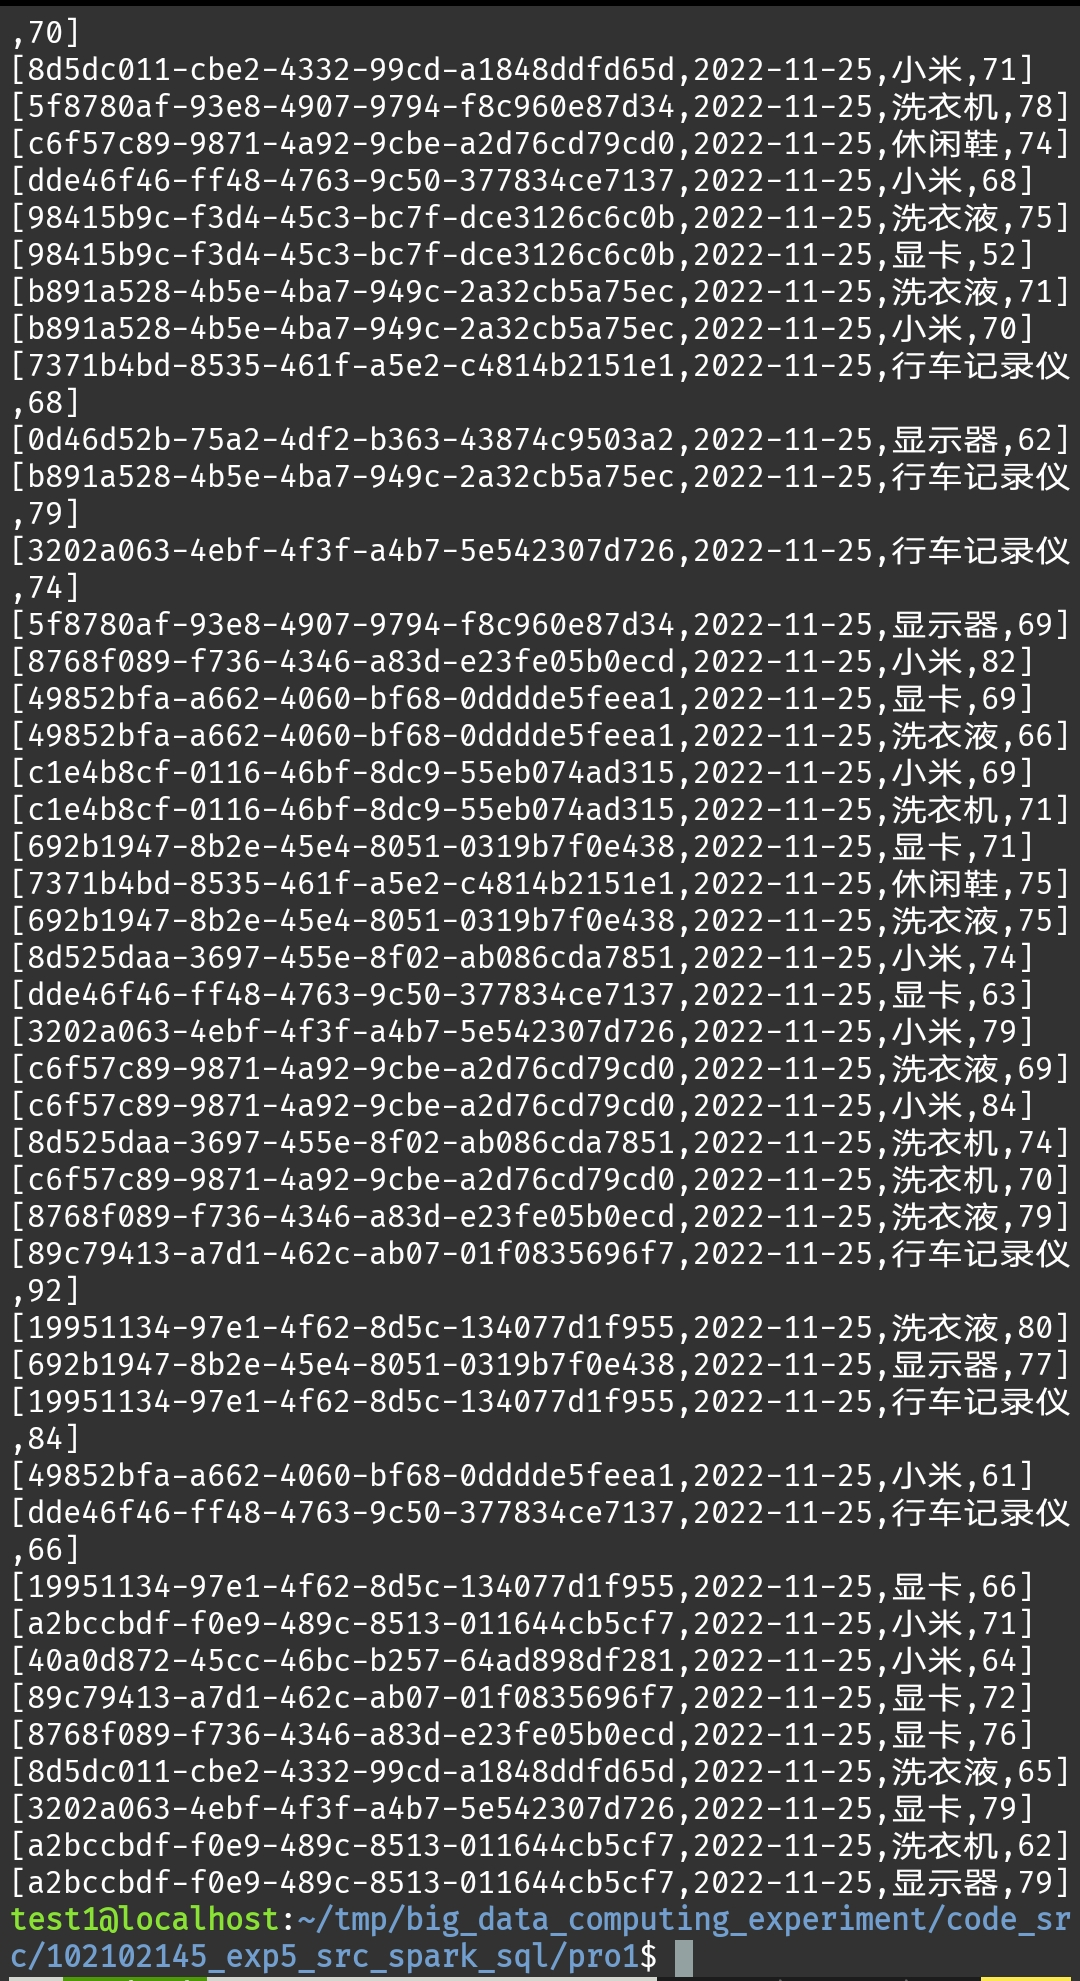
\includegraphics[width=0.65\textwidth]{./figures/3.jpg}
  \end{center}
  \caption{Running Result}
\end{figure}

\subsection{NBA 数据统计}
\subsubsection{Problem Description}
\begin{enumerate}
  \item 根据胜负场次统计 $ 15 $ - $ 16 $ 赛季都能够进入季后赛的球队
    (查询东西部联盟排名前 $ 8 $ 的球队)
  \item 针对最近两个赛季常规赛排名, 根据排名的变化, 找出东、西部进步幅度最大的球队。
  \item 分析统计出 $ 15 $ - $ 16 $ 赛季命中率(第三列)、 三分球命中率(第六列)、
    防守能力最强(失分越少防守越强)的三支球队.
\end{enumerate}

\subsubsection{Code}
\begin{center}
\begin{minted}[xleftmargin=5mm]{scala}
package net.homework

import org.apache.spark.SparkContext._
import org.apache.spark.sql.SparkSession
import org.apache.spark.sql.Row
import org.apache.spark.sql.functions.{desc, expr, row_number, col}
import org.apache.spark.sql.expressions.Window
import org.apache.spark.sql.types.{
  StructField, StructType,
  StringType, LongType, DoubleType
}

import java.nio.file.Paths

object App {
  def main(args : Array[String]) : Unit = {
    val spark = SparkSession.builder().appName("pro2").getOrCreate()

    val cwd = Paths.get("").toAbsolutePath.toString
    val inputPath = s"file://${cwd}/input"

    val schema = new StructType(Array(
      new StructField("qiudui", StringType, true),
      new StructField("saiji", StringType, true),
      new StructField("toulan", StringType, true),
      new StructField("mingzhong0", StringType, true),
      new StructField("chushou0", StringType, true),
      new StructField("sanfen", StringType, true),
      new StructField("mingzhong1", StringType, true),
      new StructField("chushou1", StringType, true),
      new StructField("faqiu", StringType, true),
      new StructField("mingzhong2", StringType, true),
      new StructField("chushou2", StringType, true),
      new StructField("lanban", StringType, true),
      new StructField("qianchang", StringType, true),
      new StructField("houchang", StringType, true),
      new StructField("zhugong", StringType, true),
      new StructField("qianduan", StringType, true),
      new StructField("gaimao", StringType, true),
      new StructField("shiwu", StringType, true),
      new StructField("fangui", StringType, true),
      new StructField("defen", DoubleType, true),
      new StructField("shifen", DoubleType, true),
      new StructField("sheng", LongType, true),
      new StructField("fu", LongType, true),
      new StructField("gongshi", DoubleType, true),
      new StructField("lianmeng", StringType, true),
    ))

    val df = spark.read
      .option("header", "true")
      .option("inferSchema", "false")
      .schema(schema)
      .format("csv")
      .load(s"${inputPath}/NBA14-16.csv")
    df.cache()
    //球队,赛季,投篮,命中,出手,三分,命中,出手,罚球,命中,出手,篮板,前场,后场,助攻,抢断,盖帽,失误,犯规,得分,失分,胜,负,公式,联盟
    //金州勇士,14-15,47.80%,41.6,87,39.80%,10.8,27,76.80%,16,20.8,44.7,10.4,34.3,27.4,9.3,6,14.1,19.9,110,99.8,67,15,81.7,west

    //\item 根据胜负场次统计 $ 15 $ - $ 16 $ 赛季都能够进入季后赛的球队
    //(查询东西部联盟排名前 $ 8 $ 的球队)
    df.where("saiji like '15%16'")
      .orderBy(desc("sheng"))
      .take(8)
      .foreach(println)
    println("======")

    //\item 针对最近两个赛季常规赛排名, 根据排名的变化, 找出东、西部进步幅度最大的球队。
    val df1 = df.withColumn("score", expr("defen - shifen"))
    val windowSpec = Window.partitionBy("saiji")
      .orderBy(col("score").desc)
      .rowsBetween(Window.unboundedPreceding, Window.currentRow)
    val df2 = df1.withColumn("rank", row_number().over(windowSpec))
    df2.createOrReplaceTempView("df2_view")
    spark.sql("""
      SELECT x.qiudui, x.rank-y.rank AS rdiff FROM
      df2_view x, df2_view y
      WHERE x.qiudui=y.qiudui AND x.saiji LIKE '14%' AND y.saiji LIKE '15%'
      """)
      .where("rdiff >= 0")
      .orderBy(desc("rdiff"))
      .take(1)
      .foreach(println)
    println("======")

    //\item 分析统计出 $ 15 $ - $ 16 $ 赛季命中率(第三列)、 三分球命中率(第六列)、
    //防守能力最强(失分越少防守越强)的三支球队.
    df.select("qiudui", "toulan", "sanfen", "shifen")
      .orderBy("shifen")
      .take(3)
      .foreach(println)
    println("======")

    spark.stop()
  }
}
\end{minted}
\end{center}

\subsubsection{Result}
\begin{figure}[H]
  \begin{center}
    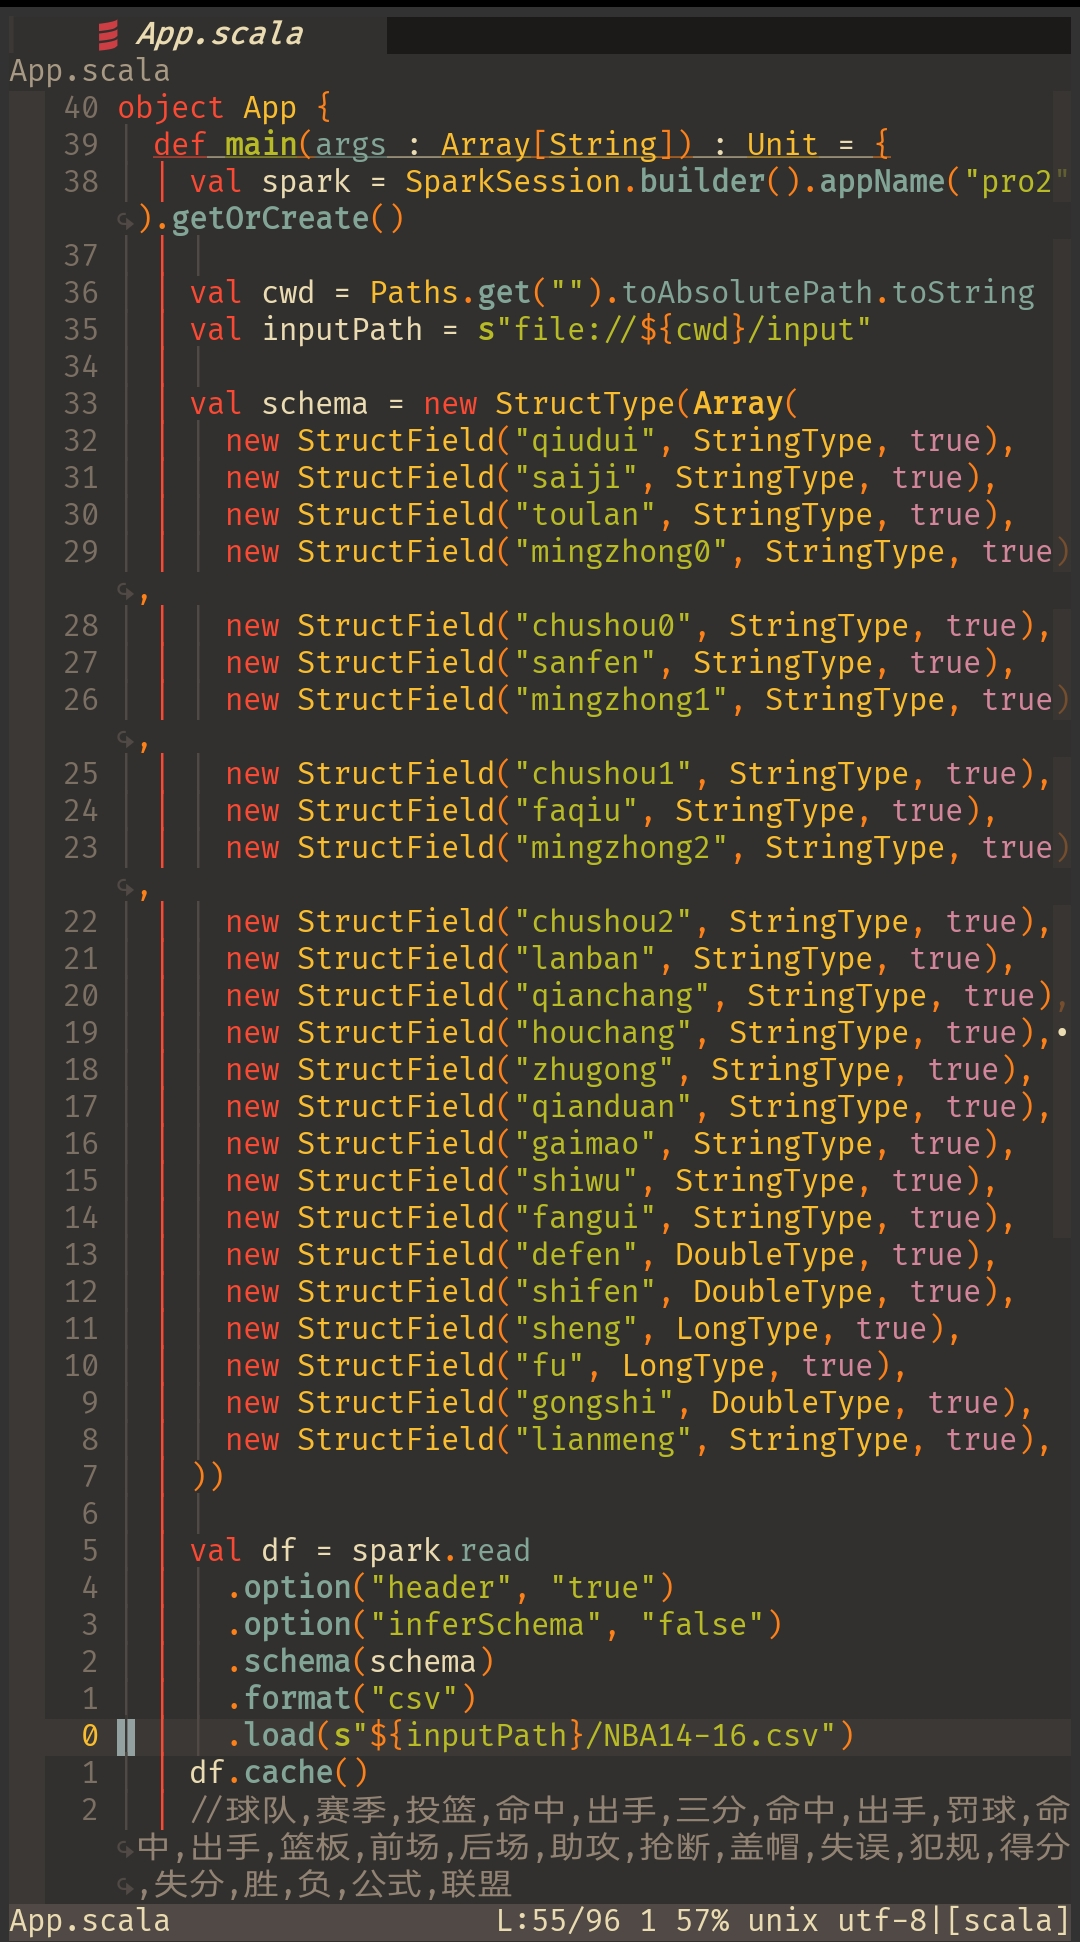
\includegraphics[width=0.65\textwidth]{./figures/4.jpg}
  \end{center}
  \caption{Code}
\end{figure}

\begin{figure}[H]
  \begin{center}
    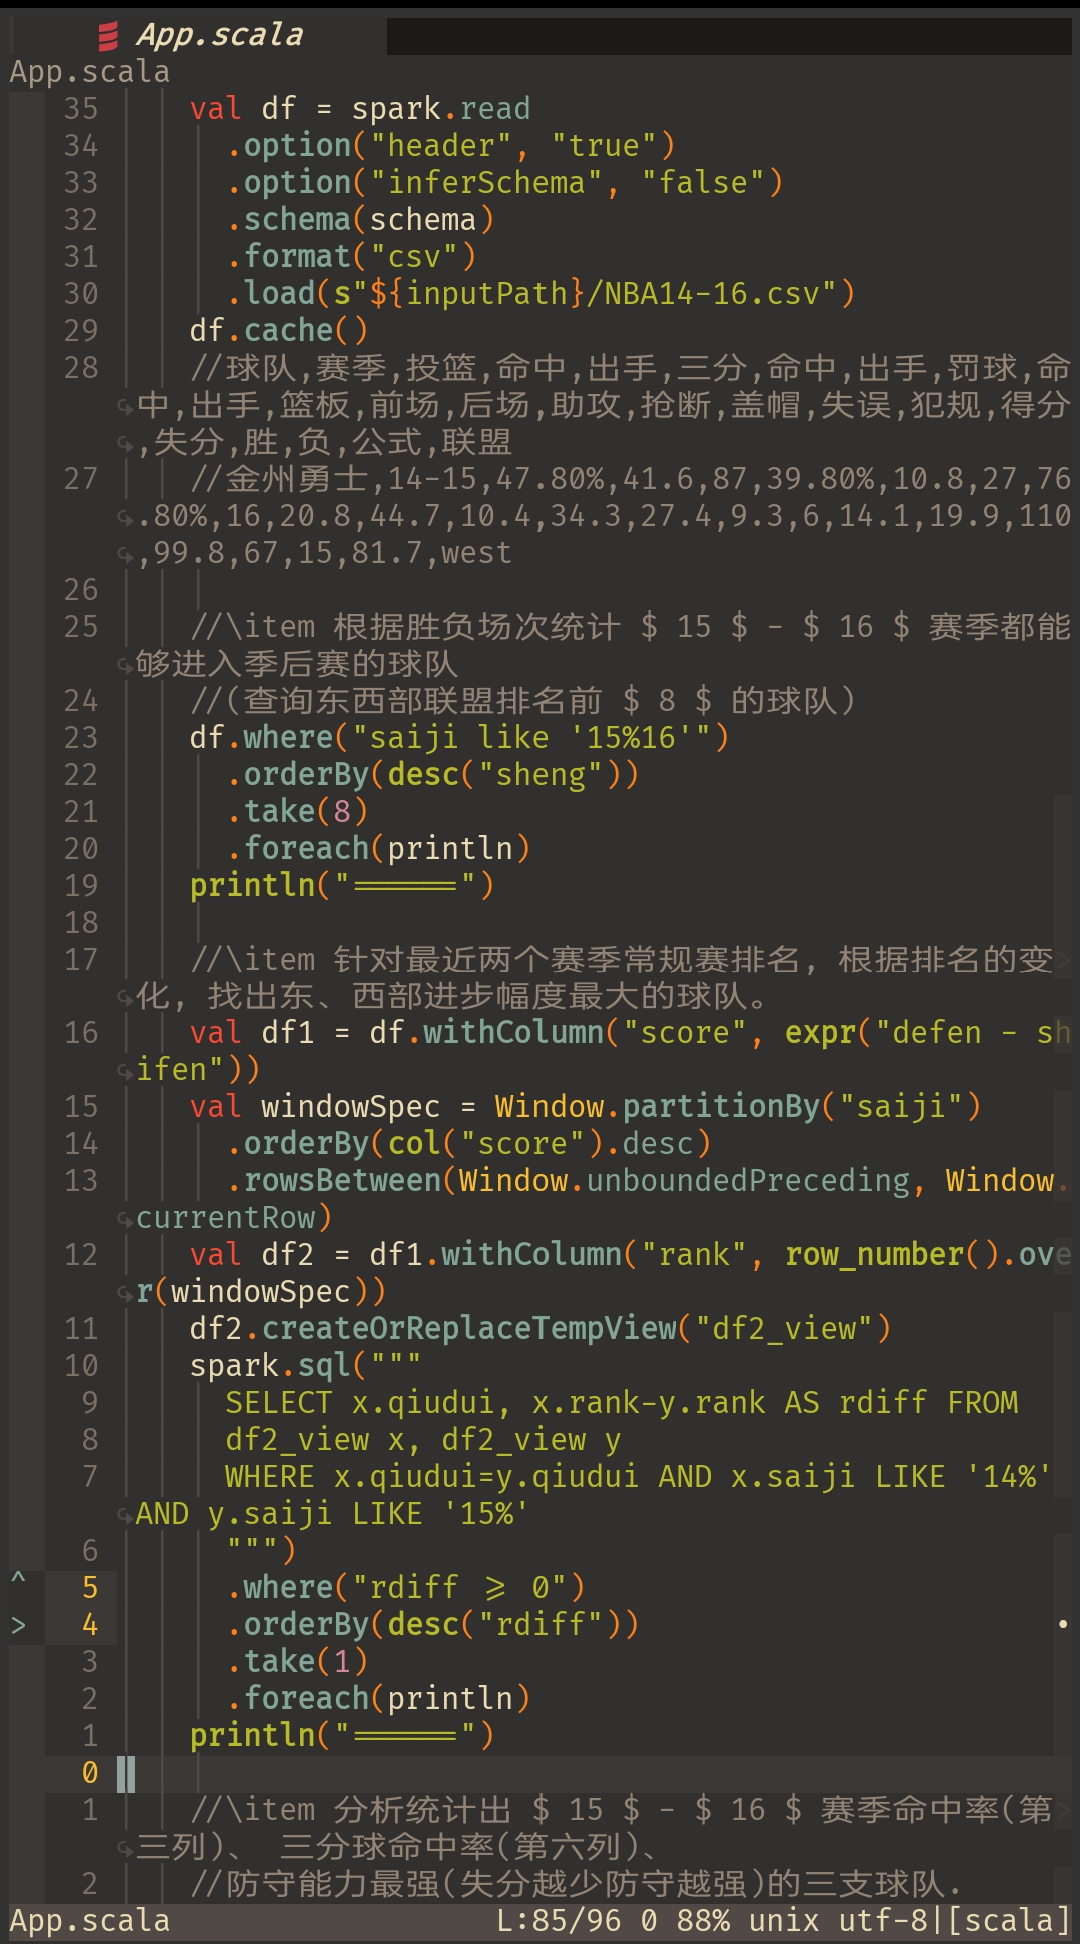
\includegraphics[width=0.65\textwidth]{./figures/5.jpg}
  \end{center}
  \caption{Code}
\end{figure}

\begin{figure}[H]
  \begin{center}
    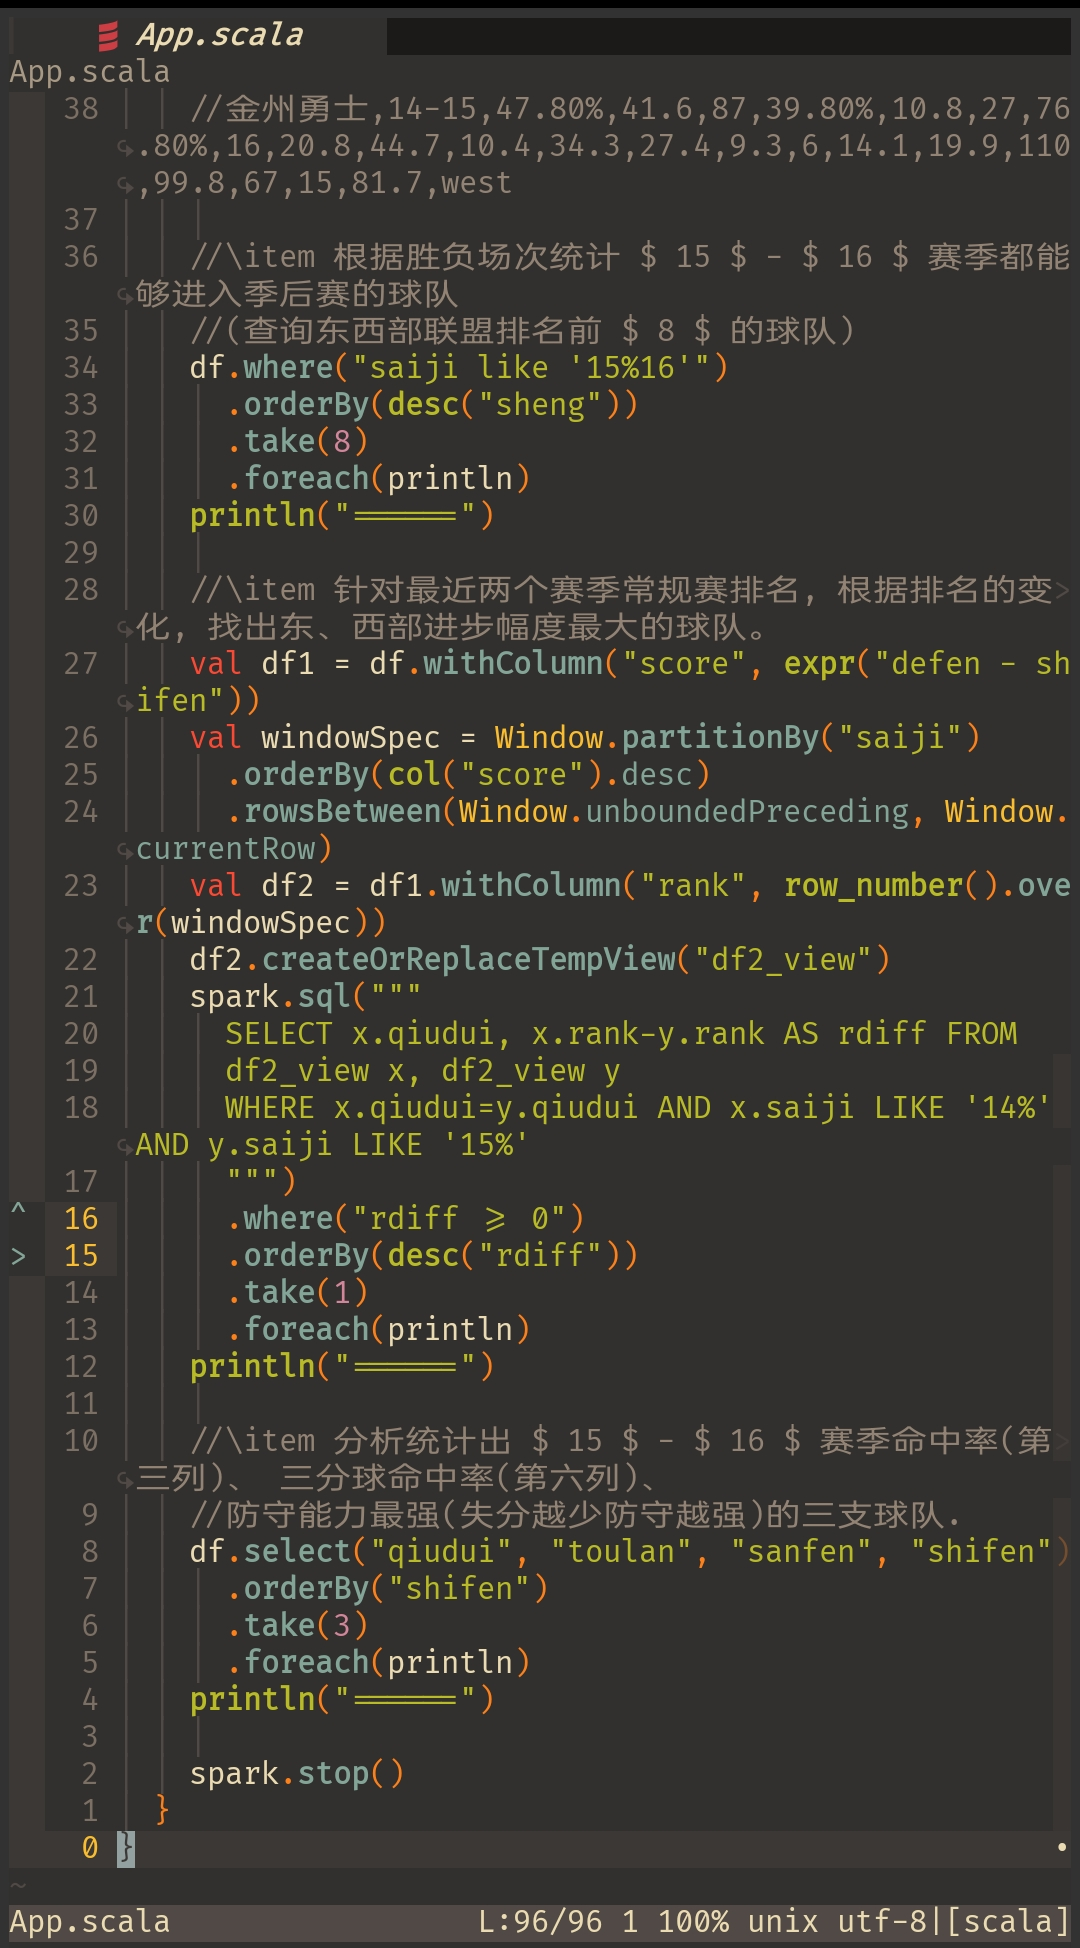
\includegraphics[width=0.65\textwidth]{./figures/6.jpg}
  \end{center}
  \caption{Code}
\end{figure}

\begin{figure}[H]
  \begin{center}
    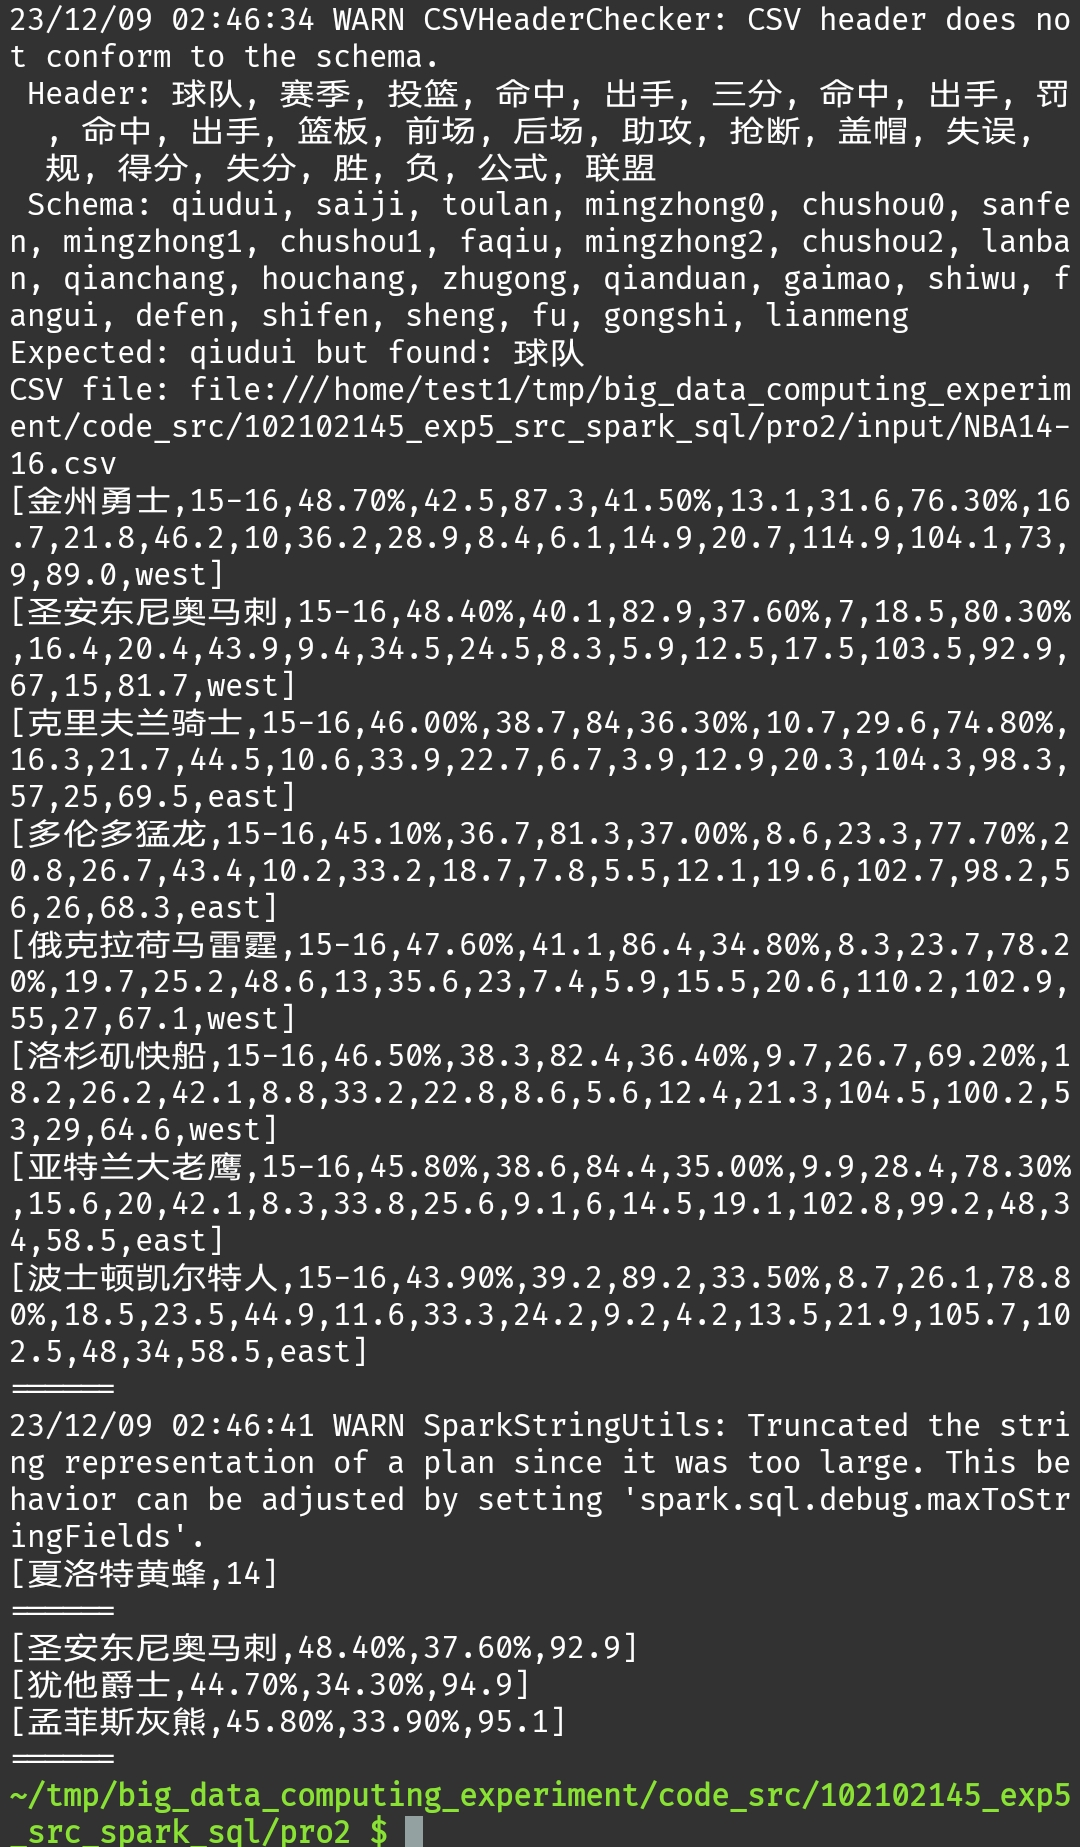
\includegraphics[width=0.65\textwidth]{./figures/7.jpg}
  \end{center}
  \caption{Running Result}
\end{figure}

\section{出现的问题及其解决方案}
没有问题.
\end{document}
